\section{Causal Identification Framework}

\subsection{The Selection Bias Problem}

A naive comparison of team performance between races where a rider is selected and races where he is not yields a biased estimate of his causal contribution. Team managers do not select riders at random: a sprinter is systematically sent to flat races and kept home for mountain stages; a domestique specialised in the high mountains is rarely chosen for cobbled classics. This endogenous selection means that the observed correlation between a rider's presence and his team's UCI points conflates the true effect of his participation with the systematic difference in race difficulty between the two groups.

Formally, let $D_i \in \{0, 1\}$ denote whether rider $r$ is selected for race $i$, and let $Y_i$ be the UCI points scored by his team on that race. A simple OLS regression of $Y_i$ on $D_i$ recovers $\mathbb{E}[Y_i \mid D_i = 1] - \mathbb{E}[Y_i \mid D_i = 0]$, which mixes the treatment effect with the difference in the covariate distribution between selected and non-selected races. Causal machine learning corrects for this bias by explicitly modelling the selection mechanism.

\subsection{Potential Outcomes and Treatment Effect}

We adopt the Rubin potential outcomes framework \citep{rubin1974}. For each race $i$, let $Y_i(1)$ be the team's UCI points if the rider is selected and $Y_i(0)$ the points if he is not. Only one of the two is observed. The quantity of interest is the \textbf{Average Treatment Effect} (ATE):
\begin{equation}
    \text{ATE} = \mathbb{E}[Y_i(1) - Y_i(0)]
    \label{eq:ate}
\end{equation}
and, more granularly, the \textbf{Conditional Average Treatment Effect} (CATE) as a function of race covariates $X_i$:
\begin{equation}
    \tau(x) = \mathbb{E}[Y_i(1) - Y_i(0) \mid X_i = x]
    \label{eq:cate}
\end{equation}
The CATE reveals for which types of races---by terrain, competition level, or team configuration---the rider's presence matters most.

\subsection{Causal DAG and Confounders}

The assumed data-generating process is represented in Figure~\ref{fig:dag}. Race characteristics $X_i$ simultaneously influence the selection decision $D_i$ and the team outcome $Y_i$. The treatment effect flows from $D_i$ to $Y_i$ along the causal arrow of interest. There is no direct arrow from $Y_i$ back to $D_i$, as selection is made before the race takes place.

\begin{figure}[H]
\centering
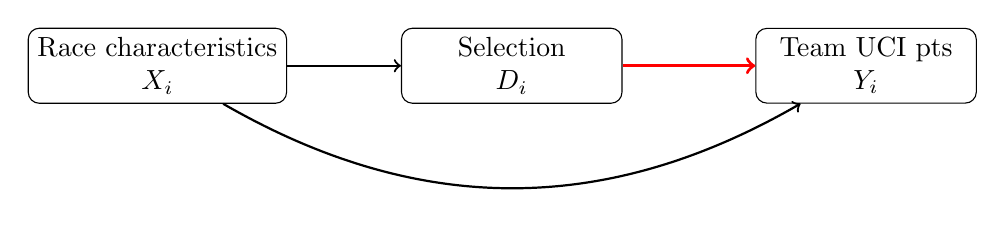
\begin{tikzpicture}[
  every node/.style={draw, rounded corners, minimum width=2.8cm, minimum height=0.8cm, align=center},
  arrow/.style={->, thick}
]
\node (X) at (0,0)   {Race characteristics\\$X_i$};
\node (D) at (4.5,0) {Selection\\$D_i$};
\node (Y) at (9,0)   {Team UCI pts\\$Y_i$};
\draw[arrow] (X) -- (D);
\draw[arrow, red, very thick] (D) -- (Y);
\draw[arrow] (X) to [bend right=30] (Y);
\end{tikzpicture}
\caption{Causal DAG. The red arrow is the effect of interest. Race characteristics $X_i$ confound both selection and outcome.}
\label{fig:dag}
\end{figure}

The covariate vector $X_i$ includes all features described in Section~3 that are observable before the race and that jointly determine selection and performance: race terrain (elevation, distance, climb profile, surface), competitive context (startlist quality, UCI classification), team dynamics (rolling form by stage type, presence of the team's designated leader, whether the rider himself is the team's top scorer), and the rider's recent workload.

\subsection{Identification Assumptions}

Identification of the ATE and CATE rests on three standard assumptions.

\textbf{Conditional independence} (unconfoundedness): given the observed covariates $X_i$, the potential outcomes are independent of the treatment assignment:
\begin{equation}
    (Y_i(0), Y_i(1)) \perp\!\!\!\perp D_i \mid X_i
    \label{eq:cia}
\end{equation}
This holds if $X_i$ captures all variables that simultaneously influence selection and outcome. The rich feature set described in Section~3 is designed precisely to satisfy this condition.

\textbf{Overlap}: every race has a strictly positive probability of being in either group:
\begin{equation}
    0 < \mathbb{P}(D_i = 1 \mid X_i = x) < 1 \quad \forall x
    \label{eq:overlap}
\end{equation}
Riders with very few non-selected observations in certain race types would violate this assumption. The inclusion criteria of at least 30 selected and 30 non-selected observations (Section~2) serve as an empirical safeguard.

\textbf{SUTVA} (Stable Unit Treatment Value Assumption): the potential outcomes of race $i$ do not depend on the selection status of other races. This is satisfied here since each (rider, race) pair is treated as an independent observation.

\subsection{Outcome Variables}

Two levels of analysis are defined, corresponding to two distinct data structures.

At the \textbf{stage level}, the outcome is the UCI points scored by the rider's team on a single stage: $Y_i = \texttt{pts\_uci\_equipe\_stage}$. This is the primary outcome. Each observation corresponds to one (rider, stage) pair.

At the \textbf{race level}, the outcome is the UCI points scored by the team in a classification standing at the end of a multi-day race: general classification ($\texttt{pts\_uci\_equipe\_gc}$), mountain classification ($\texttt{pts\_uci\_equipe\_kom}$), or sprint classification ($\texttt{pts\_uci\_equipe\_points}$). These outcomes cannot be modelled at the stage level since the points are awarded once per race. Each observation corresponds to one (rider, race) pair, and the model uses race-level aggregates of the stage features (sums for cumulative features such as elevation; first observation for contextual features such as team form).
